\documentclass[11pt]{standalone}
\usepackage{tikz, pgfplots,amsmath, amssymb, amsthm}   
\usepgfplotslibrary{groupplots}


\begin{document}


  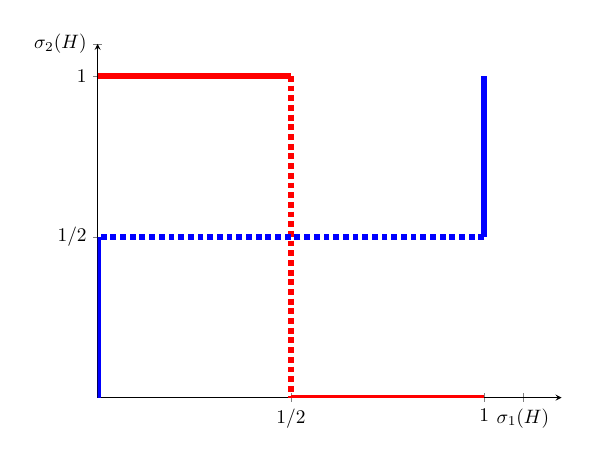
\begin{tikzpicture}[scale=.7]


\begin{axis}[
  height=8cm, width=10cm,
  axis x line=bottom, axis y line=left,
  ymin=0, ymax=1.1, xmin=0, xmax=1.2,
  xtick={0.5,1,1.1},
  xticklabels={1/2,1,$\sigma_1(H)$},
  ytick={0.5,1,1.1},
yticklabels={1/2,1,$\sigma_2(H)$},
]
    
%\addplot[black scatter,only marks, scatter src=explicit symbolic]  coordinates {(5, 5)} node[anchor=north] {$p^*$};

\node at (axis cs:12, 5) [anchor=south west] {A};
\node at (axis cs:20,11) [anchor=north west] {B};





\draw [line width=3pt,draw=red,fill=none, opacity=1] (axis cs:0, 1) -- (axis cs:0.5, 1) ;
\draw [line width=3pt,dotted,draw=red, fill=none, opacity=1] (axis cs:0.5, 1) -- (axis cs:0.5, 0) ;
\draw [line width=3pt,draw=red, fill=none, opacity=1] (axis cs:0.5, 0) -- (axis cs:1, 0) ;
\draw [line width=3pt,draw=blue,fill=none, opacity=1] (axis cs:1, 0.5) -- (axis cs:1, 1) ;
\draw [line width=3pt,dotted,draw=blue, fill=none, opacity=1] (axis cs:1,0.5) -- (axis cs:0, 0.5) ;
\draw [line width=3pt,draw=blue, fill=none, opacity=1] (axis cs:0, 0) -- (axis cs:0, 0.5) ;
\end{axis}

 \end{tikzpicture}



\end{document}\textbf{}\textbf{}